\section{Pozorování v latentním prostoru}
\label{sec:vae_model_latent_space_observation}

Po natrénování modelu variačního autoenkodéru lze nahlédnout do zformovaného latentního prostoru.
Jednotlivé body latentního prostoru jsou tvořeny průchodem vstupních dat (MNIST číslic) enkodér modulem.
\autoref{fig:vae_model_latent_space} ukazuje jejich obarvení, které bylo přiřazeno na základě třídy vstupního vzorku (tedy v tomto případě má každá číslice $0$ - $9$ přiřazenou jednu barvu)\footnote{Pro vizualizaci 2D latentního prostoru MNIST číslic je výsledná vizualizace srovnatelná s výsledky obdrženými využitím t-SNE techniky, které prezentuje \textcite{Hinton2002}.}.


\begin{figure}[H]
    \centering
    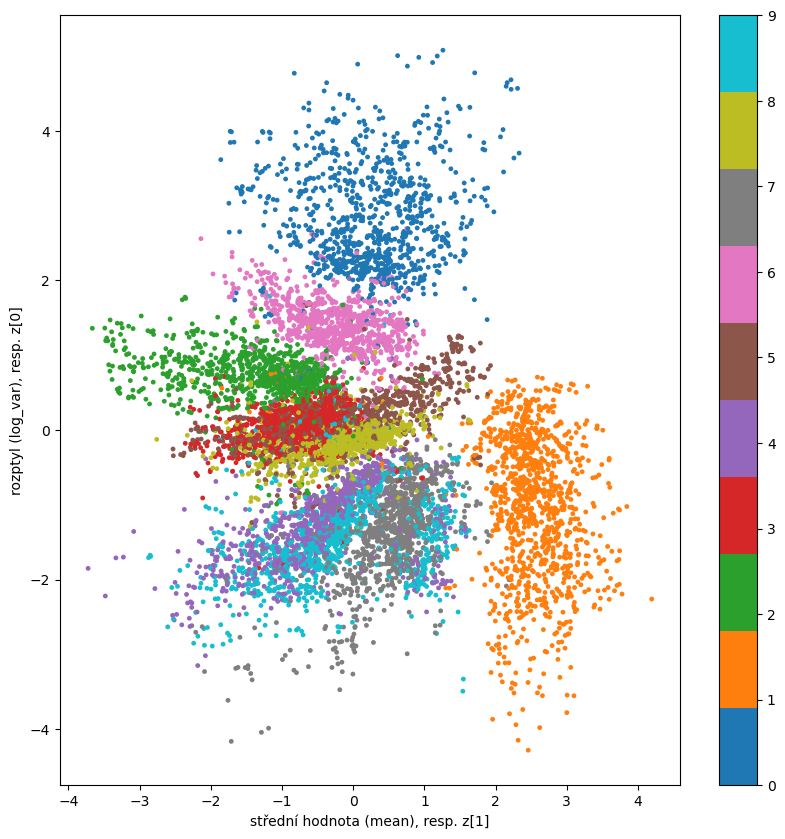
\includegraphics[width=0.95\textwidth]{figures/vae_model_latent_space_500_epochs.png}
    \caption{Latentní prostor naučeného modelu variačního autoenkodéru. Barvy reprezentují jednotlivé třídy MNIST datasetu. Celkový počet zobrazených latentních proměnných je $10 000$.}
    \label{fig:vae_model_latent_space}
\end{figure}

Latentní prostor je organizovaný, \textbf{i přes to, že model variačního autoenkodéru neměl k dispozici štítky trénovacích dat}. 
Tyto uskupení jsou důsledkem ztrátové funkce modelu.
\textbf{Variační autoenkodér se sám naučil tvar a charakteristiky jednotlivých číslic} minimalizací chyby rekonstrukce.

Zároveň vzdálenost mezi skupinami číslic, jejichž vzorky jsou si \emph{podobné} (např. $4$ a $9$) má v latentním prostoru naučeného modelu tendenci být nízká.
I proto lze u naučeného modelu pozorovat určitý sémantický význam aritmetiky v latentním prostoru (např. \emph{plynulý přechod} při posunu mezi $0$ a $9$).

\subsection{Postupné formování latentního prostoru}
\label{sec:latent_space_development}
\autoref{fig:forming_latent_space} zachycuje vliv počtu epoch trénovací fáze na strukturu latentního prostoru naučeného modelu.
S rostoucím počtem epoch lze pozorovat emergenci oddělených uskupení latentních proměnných, kdy každé takové uskupení zachycuje jednu z tříd MNIST datasetu (tedy číslice 0 - 9).

\begin{figure}[H]
    \centering
    \subfloat[Počet epoch $ = 1$.]{{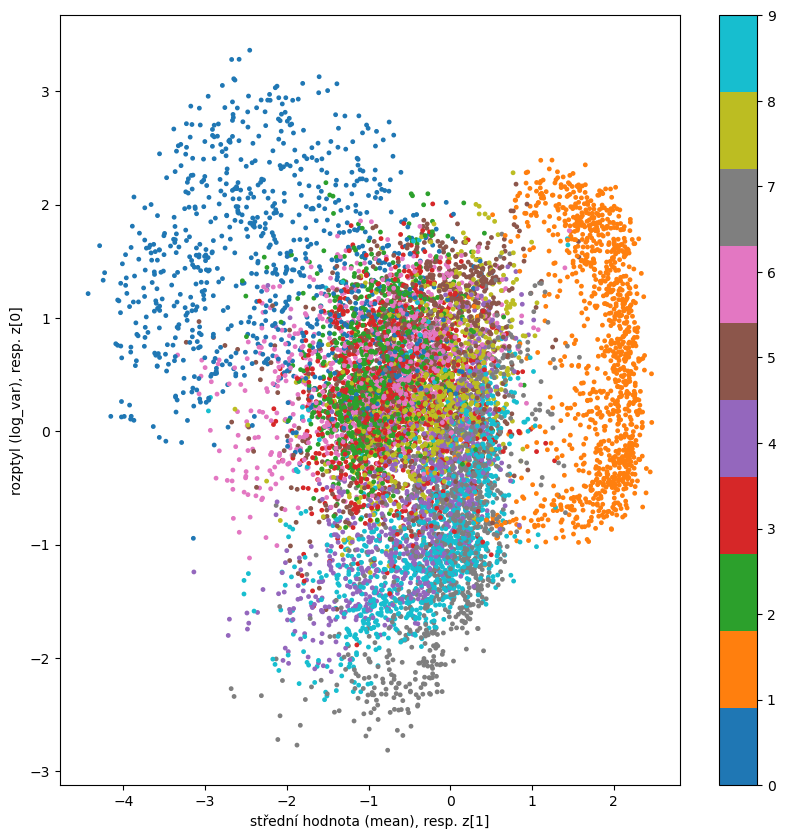
\includegraphics[width=0.49\textwidth]{figures/vae_model_latent_space_1_epoch.png} }}
    \subfloat[Počet epoch $ = 5$.]{{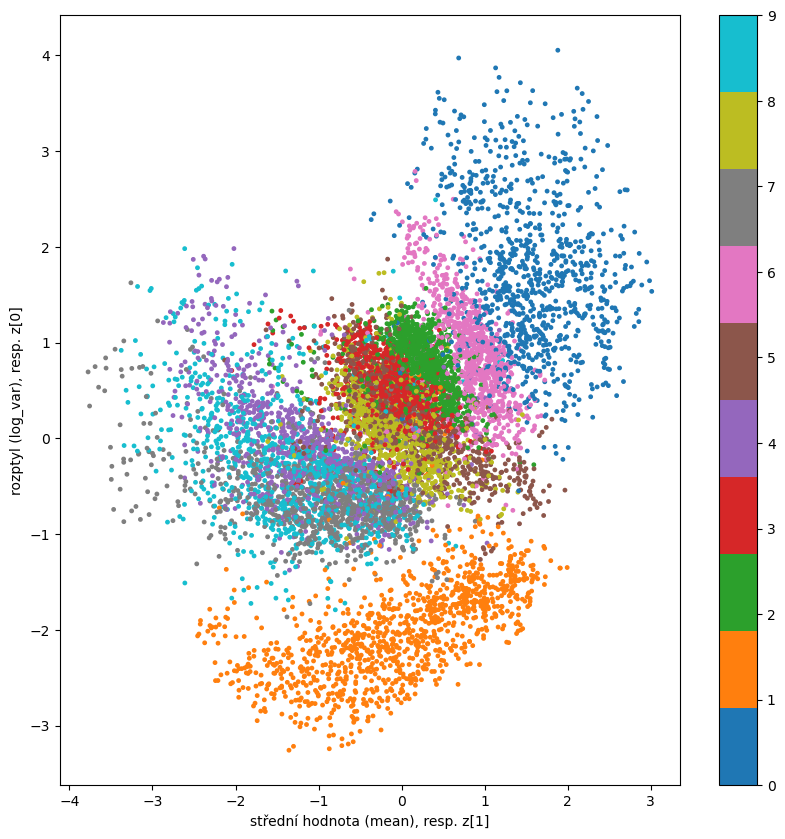
\includegraphics[width=0.49\textwidth]{figures/vae_model_latent_space_5_epochs.png} }} \\
    \subfloat[Počet epoch $ = 200$.]{{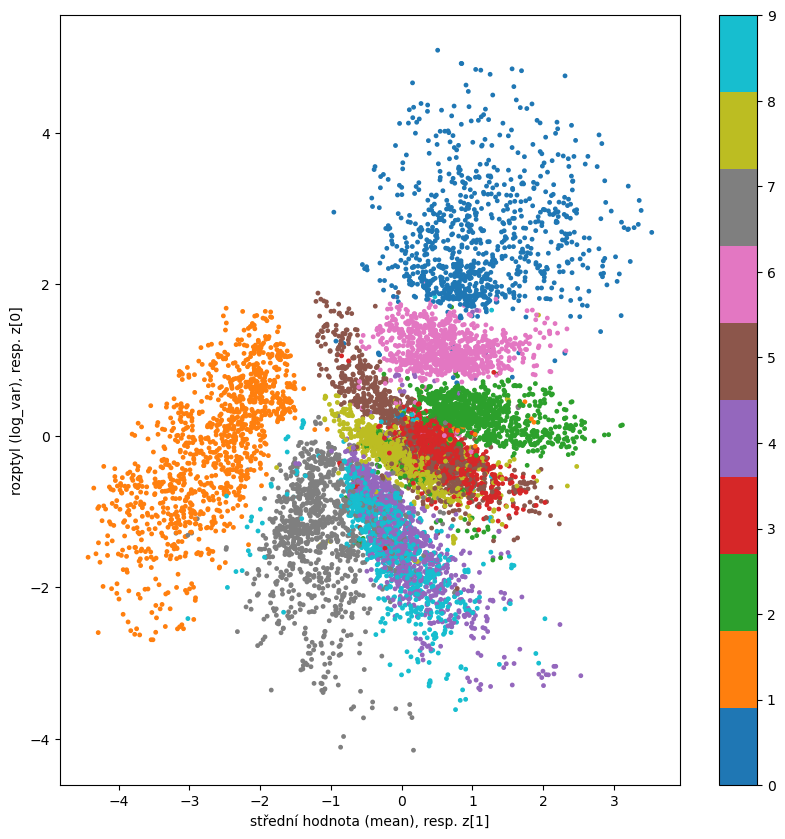
\includegraphics[width=0.49\textwidth]{figures/vae_model_latent_spac_200_epochs.png} }}
    \subfloat[Počet epoch $ = 500$.]{{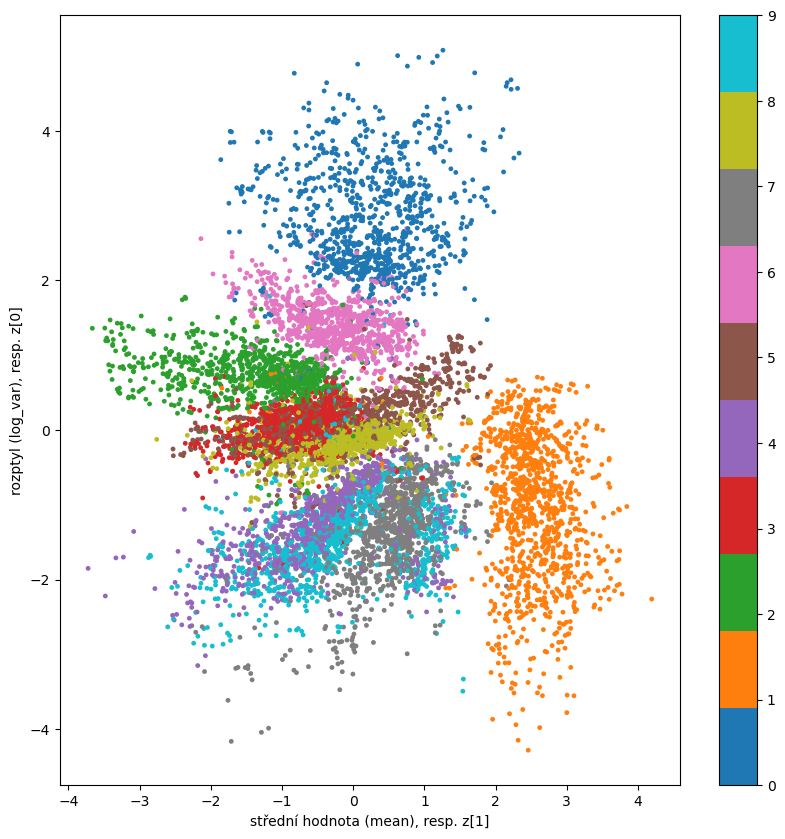
\includegraphics[width=0.49\textwidth]{figures/vae_model_latent_space_500_epochs.png} }}
    \caption{Postupné formování struktur v latentním prostoru naučeného modelu pro generativní modelování MNIST číslic.
    Dílčí obrázky a, b, c, d zachycují výsledný latentní prostor modelu, jehož trénovací fáze zahrnovala 1, 5, 200, 500 epoch respektive.
    Při trénování jednotlivých modelů byla využita pouze trénovací trénovací množina MNIST datasetu \textbf{bez štítků}.
    \textbf{Parametry vizualizace jsou pro každý dílčí obrázek identické} a liší se pouze počtem epoch, kterými model v trénovací fázi prošel.
    }
    \label{fig:forming_latent_space}
\end{figure}

Lze pozorovat, že model na \autoref{fig:500_epochs} po dodatečných 300 epochách trénování oproti \autoref{fig:200_epochs} dospěl k defacto zrcadlovému zobrazení bodů v latentním prostoru. To vedlo k snížení absolutní hodnoty ztrátové funkce o 2 body, tedy zřejmě se tato změna ve formování latentního prostoru pojí s určitým skrytým významem pro zpřesnění rekonstrukce.
Hodnoty ztrátové funkce jednotlivých modelů zachycuje PŘÍLOHA X.